\documentclass{article}
\usepackage[utf8]{inputenc}
\usepackage[margin = 0.8in]{geometry}
\usepackage{graphicx}
\usepackage{amsmath, amssymb}
\usepackage{subcaption}
\usepackage{multirow}
\usepackage{mathtools}
\usepackage{float}


\title{RBE595 - Week 6 Assignment}
\author{Keith Chester}
\date{Due date: February 19, 2023}

\begin{document}
\maketitle

In this assignment, we looked at a simple stochastic environment of 6 consecutive cells, labeled 0 through 4. Either end of the line of cells were terminal states - cell 0 with a reward of 1, cell 5 with a reward of 5. All other cells were a reward of 0 with a choice to go either left or right. There existed an 80\% chance of the robot in our environment following the designated action, a 15\% chance of the robot merely staying where it is, and a 5\% chance for the robot to go the opposite of what was chosen.

Here we developed two Monte Carlo agents - an exploring starts agent and a first visit agent. We looked at the convergence of the agent at the end of a set number of episodes, from 1 episode to 500 episodes. For each of these episodes, we performed the test with 100 different agents. We then looked at the average Q value of each state/action pair.

\begin{figure}
    \centering
    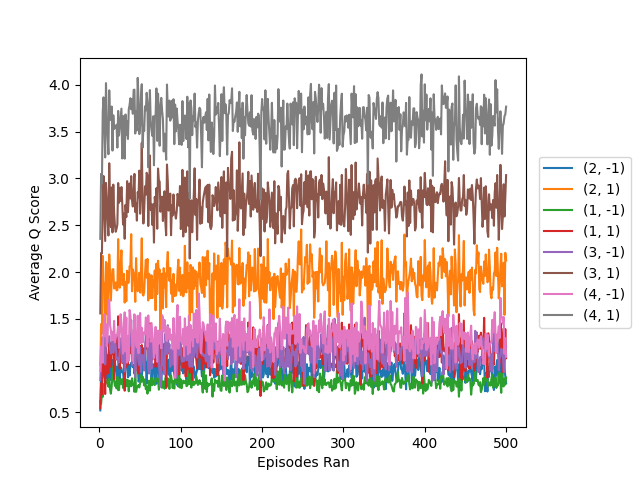
\includegraphics[width = 0.8\textwidth]{results_exploring_start.png}
    \caption{Q Value Avg for Exploring Starts Monte Carlo Agent}
\end{figure}

\begin{figure}
    \centering
    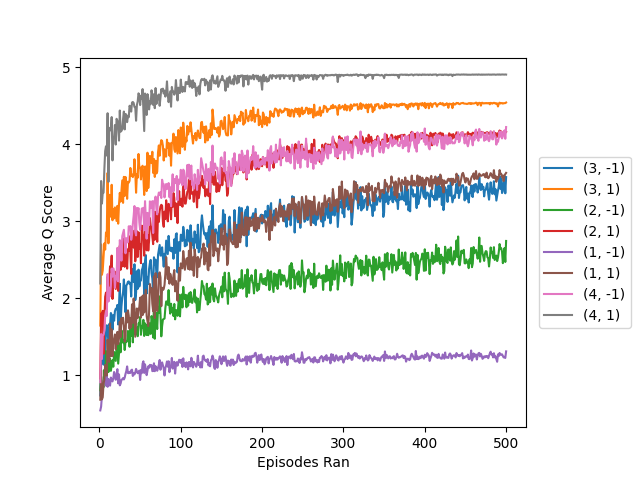
\includegraphics[width = 0.8\textwidth]{results_first_visit.png}
    \caption{Q Value Avg for First Visit Monte Carlo Agent}
\end{figure}




\end{document}
